\documentclass[12pt,a4paper]{article}
\usepackage[top=2cm,bottom=2.5cm,left=3cm,right=1.5cm]{geometry}
\usepackage[T1]{fontenc}
\usepackage[utf8]{inputenc}
\usepackage{newtxtext,newtxmath}
\usepackage{graphicx,longtable,array,booktabs,amsmath}
\usepackage[hidelinks]{hyperref}
\usepackage{caption}
\captionsetup{font=normalsize}
\setlength{\parindent}{1.25cm}
\setlength{\parskip}{0pt}
\sloppy
\begin{document}
\noindent DOI: [assigned by the editors]\par
\noindent\textbf{Mukhammed Zhumali}\par
\noindent 262937@astanait.edu.kz\par
\noindent [AUTHOR TO COMPLETE: degree, position, department, organization, country, ORCID]\par
\begin{center}\textbf{When Future Contacts Improve Satellite Key and Security Association Management}\end{center}
\textbf{Abstract:} Short satellite contacts must carry payload and the operations needed to use valid traffic keys. A longer view of future contacts can help only if it changes a feasible plan and the controller can find and execute that plan in time. This study asks when that extra view improves joint key and security association management. We compare two horizons with the same actions, safety rules, costs, and five ordered service and resource criteria. Exact search is limited to a finite event model; a practical controller uses seeds, retained plans, and bounded search. New registered tests comprise 110 full controller attempts and twelve paired root diagnostics, separate from the prior campaign. Of the controller attempts, 105 finish and five stop with incomplete search. In a nine case synthetic family, the longer horizon serves one extra contact in two cases under both tie rules. Five cases tie and two remain unresolved. Matching the initial state shows that common key preparation removes one exact versus practical gap. In the autonomous case, a useful continuation is valid but lies beyond the practical node budget. Increasing the budget gives no offline horizon gain in the two tested workloads. Charging measured decision time makes the longer horizon worse in three of four pairs. Across 36 key disclosure runs, earlier recovery and extra confidential delivery depend on the tie rule. Early key activation can also expire before any later delivery. These results support a conditional scheduling benefit, not a general security or performance advantage. They identify validity, available window length, computation, and plan selection as limits on its practical value.

\textbf{Keywords:} satellite security, key lifecycle, contact planning, computation, recovery

\section*{Introduction}
Short spacecraft--ground contacts must accommodate both payload transmission and the management of traffic keys and security associations. A later contact may provide enough time to transmit its payload but insufficient time to establish the required security state. Earlier preparation can therefore matter, provided that validity, authorization, resource availability, and communication constraints permit it. Established space-security standards already define protection and management mechanisms [1] [2] [3]; the operational question is when to invoke their abstract counterparts.

Predictable connectivity also supports routing over planned contacts [4] [5]. However, a longer forecast does not itself establish a useful scheduling advantage. A feasible improvement may require a particular initial state, a suitable return contact, and enough computation to discover and execute the plan. Decision time can consume the communication opportunity that the plan seeks to preserve.

This study examines the incremental value of contact visibility for joint traffic-key and security-association lifecycle timing. Matched Next and Multi policies use the same actions, constraints, objective, costs, and tie-breaking rule, while observing different horizons. The analysis separates exact finite-model results from practical bounded execution, without assuming that additional visibility improves service.

\section*{Literature review and problem statement}
Several established mechanisms already connect security management to intermittent or predicted connectivity. The expired Delay-Tolerant Key Administration proposal proactively distributes authenticated public keys using planned communications and effective times [6]. BERMUDA addresses unicast key management for delay-tolerant networks through public-key infrastructure, elliptic-curve key agreement, and certificate revocation [7]. These works concern the availability and administration of cryptographic material; they prevent treating advance preparation as a new mechanism.

Satellite handover research provides another precedent. Zhao transfers authentication context and session-key information before a predicted handover [8]. Kwon et al. separate initial authentication from lightweight handover operations in a satellite--terrestrial architecture [9]. Such designs establish that anticipating mobility and reducing repeated authentication costs are existing research directions.

Bernal et al. provide a particularly relevant contact-dependent identity architecture [10]. Ground-side identity operations support onboard authorization allowlists updated during satellite contacts. Their discussion also includes revocation delay, temporary local authorization withdrawal, and short-lived capability tokens. Thus, this work already couples authorization state to intermittent connectivity. The distinction considered here is the timing of directional traffic keys and security associations across an ordered contact sequence, rather than device identity or ledger-backed authorization.

Bundle Protocol Version 7 and BPSec establish a separate networking and security context [11] [12]. Most directly, Detke et al. translate temporally feasible Contact Graph Routing routes into protection-scheme-dependent key scopes and minimize the activated scopes needed for a target connectivity ratio [13]. Their model addresses route feasibility and provisioning footprint; scheduling keys over contact plans is identified as a further direction. The present study instead examines sequential lifecycle actions and their effects on admissible payload service under fixed constraints.

Receding-horizon optimization is itself established [14]. The narrower problem is whether changing only the visible contact horizon changes the selected lifecycle schedule, and whether a practical controller can realize that change within its computational budget. This operational comparison neither supplies a new authentication protocol nor substitutes for cryptographic analysis such as formal BPSec studies [15]. Consequently, any contribution must remain conditional on the modeled state, workload, constraints, and execution method.

Related work also addresses BPSec security models and policies [16]. Concrete contexts specify cryptographic processing and key-use rules [17]. Our abstract operations are inspired by lifecycle requirements; the simulator implements neither those BPSec contexts nor a certified implementation of the space data-link standards. Its evidence concerns operation timing and modeled consequences, not protocol-level cryptographic strength.

\section*{Aim and objectives}
The research question is: under identical lifecycle actions, security constraints, costs, and plan tie-breaking, when does additional predicted contact visibility improve achievable spacecraft--ground service, and when can a bounded receding-horizon controller realize that improvement?

The hypothesis is conditional: a longer horizon can expose a later contact whose service requires an earlier key or security-association operation, allowing a contact to be served that the shorter-horizon schedule misses. The effect can disappear when later time is sufficient, old material remains valid, search cannot discover the continuation, or computation consumes the useful opportunity.

The objectives are to isolate initialization from search, test source-derived timing and validity conditions, measure full-run quality under fixed computational budgets, and separate stages of recovery after key disclosure. The contribution is a joint lifecycle scheduling formulation and evidence locating its useful and ineffective regimes. Conditional model properties support interpretation; implementation checks support reproducibility rather than constituting a separate claim of scientific novelty.

\section*{Materials and methods}
\subsection*{State and admissible execution}
A contact specifies a spacecraft, ground station, start, end, and offered payload in each direction. Each station context holds directional traffic-key material, installation acknowledgments, active generations, security associations, and counters. Key creation, installation, activation, and association opening are distinct events. PREPARE creates a pair; INSTALL confirms its availability at both ends; SWITCH activates it; OPEN or REUSE opens a context with admissible material. CONTINUE sends one complete frame; WAIT advances to an event without starting another frame. STOP and EXPIRE follow the executor rules automatically. One spare candidate and shared resources restrict the action space.

A material-age bound A is measured from creation c, and a cryptoperiod P from successful activation a. Previously committed deadlines cannot be extended by later opening or reuse. The use deadline d is bounded as in (1), with absent terms omitted before activation. Authorized context, directional binding, installation, acknowledgment, counters, and validity throughout a frame are checked in addition to this time bound.

\begin{equation}d=\min\{c+A,\ a+P,\ d_{\mathrm{committed}}\}\tag{1}\end{equation}
Management operations occupy elapsed time and, when applicable, the shared radio. The profile records spacecraft and ground CPU separately, radio occupancy, and uplink/downlink management bytes. Operations interrupted by a boundary charge only the executed phases; useful time includes complete delivered payload frames. The synthetic profile used in the new tests is summarized in Table 1. These are model parameters, not flight-hardware benchmarks. Search CPU and host elapsed time are measured separately.

\begin{longtable}{>{\raggedright\arraybackslash}p{5.42cm}>{\raggedright\arraybackslash}p{3.16cm}>{\raggedright\arraybackslash}p{3.16cm}>{\raggedright\arraybackslash}p{3.16cm}}
\caption*{Table 1. Synthetic operation profile; CPU is spacecraft plus ground, bytes are both directions.}\\
\toprule
\textbf{Operation} & \textbf{Elapsed (s)} & \textbf{CPU (s)} & \textbf{Bytes}\\\midrule\endfirsthead
\textbf{Operation} & \textbf{Elapsed (s)} & \textbf{CPU (s)} & \textbf{Bytes}\\\midrule\endhead
PREPARE & 2 & 0.20 & 0\\
INSTALL & 4 & 0.30 & 800\\
SWITCH & 1 & 0.15 & 200\\
OPEN / REUSE & 1 & 0.06 & 80\\
Revocation notice & 0.4 & 0.04 & 96\\
\bottomrule\end{longtable}
\subsection*{Objective and matched policies}
A contact is served once its required uplink and downlink delivery thresholds are both met. A root evaluation includes the current contact's already delivered progress and counts only incremental reward and costs, with no double counting of completed preparation. The five ordered criteria in (2) maximize served contacts S and useful payload time U, then minimize modeled operation CPU C, management bytes B, and newly created directional keys K. One extra served contact outranks any loss of useful time or increase in cost. Risk is not minimized by this objective.

\begin{equation}\operatorname{maximize}_{\mathrm{lex}}\ J=(S,U,-C,-B,-K)\tag{2}\end{equation}
Next uses H=1 and Multi H=2, where H counts future contacts beyond the current one. Inside C1, Next observes C1 and C2, while Multi also observes C3. Between contacts, H nearest contacts are available. Visible contacts, payload, and evaluationEnd remain fixed during a search; moving to another contact inside a branch reveals nothing new. The endpoint is the last visible contact's end. Future attacks and failures are excluded from the observation.

Both horizons use the same finite start-event set, executor, constraints, resource model, generation identifiers, traversal, and score comparator. Only after all five criteria tie is a full-plan order applied. CANONICAL is the original operation/identifier order. CONTINUE\_WAIT prefers CONTINUE, then WAIT, then service operations, followed by the same deterministic identifier and timing fields. Changing traversal alone would not change this final tie order. Canonical pruning and retained-plan selection use the selected comparator.

The exact solver explores the finite admissible continuations with validated pruning and state reuse. COMPLETE certifies this model's root optimum, including tie order; a time or node stop is INCOMPLETE. The controller executes the first action and replans at events, except for an already proved continuation after a guarded nominal frame. Root optimality does not prove whole-mission optimality. The practical controller compares feasible seeds, retained continuations, and bounded-search results. FINISHED means that execution reached its endpoint, not that every decision was proved optimal.

\subsection*{Registered experiments and provenance}
All new experiments used a separate harness against the unchanged Java 21 final-v2 JAR. They comprise 110 new full-controller attempts and twelve paired-root diagnostics; six identical cells are reused with explicit origin links. These are separate from the preserved 108-attempt baseline campaign, which has 93 FINISHED and 15 PROCESS\_TIMEOUT outcomes. Table 2 gives the new denominators. Every registered attempt was run; limits were not increased after an unsuccessful result.

\begin{longtable}{>{\raggedright\arraybackslash}p{5.81cm}>{\raggedright\arraybackslash}p{1.79cm}>{\raggedright\arraybackslash}p{2.5cm}>{\raggedright\arraybackslash}p{2.86cm}>{\raggedright\arraybackslash}p{1.79cm}}
\caption*{Table 2. Registered new attempts and completion; reused cells are not new attempts.}\\
\toprule
\textbf{Block} & \textbf{New} & \textbf{Finished} & \textbf{Unfinished} & \textbf{Reused}\\\midrule\endfirsthead
\textbf{Block} & \textbf{New} & \textbf{Finished} & \textbf{Unfinished} & \textbf{Reused}\\\midrule\endhead
Matched initial states & 16 & 15 & 1 & 0\\
Synthetic conditions & 32 & 28 & 4 & 4\\
Computational budgets & 26 & 26 & 0 & 2\\
Key disclosure & 36 & 36 & 0 & 0\\
Controller total & 110 & 105 & 5 & 6\\
Paired-root diagnostics & 12 & 11 complete & 1 incomplete & 0\\
\bottomrule\end{longtable}
Exact searches allow 2,000,000 nodes and 30 seconds per decision. Practical searches allow 5,000 nodes and one second, with a two-second decision allowance, 350 milliseconds each for seed and retained-plan evaluation, and 10,000 rollout transitions. Full controllers have a 120-second host budget and a separate 150-second process watchdog; root diagnostics have a 60-second watchdog. One JVM runs at a time with a 1 GiB heap. An isolated incumbent logger is used only in root diagnostics and checked against the frozen planner on a complete fixed-node control. Its elapsed times include instrumentation overhead.

The synthetic family uses C1 at A from 0 to 20 seconds, C2 at B from 30 to 50, and C3 at A from T to T+L. X01 has T=80, L=5, and P=150 seconds. Common preparation runs from $-$2 to 0 and its costs remain in the journal; autonomous runs start without a spare pair. Initial A material was created at $-$90 and activated at $-$80, and B at $-$40 and $-$30. Material age is 400 seconds and maximum reuse gap 200 seconds. Changing P rebuilds history through lifecycle transitions; expiry is never edited independently.

The remaining family settings are shown in Fig. 1. At 100 bytes per frame and 400 bytes per second, each frame lasts 0.25 seconds; the two directional thresholds of 400 bytes require eight frames, or two seconds. A pre-active installed pair therefore needs SWITCH+OPEN+payload, four seconds, while a prepared pair needs INSTALL+SWITCH+OPEN+payload, eight seconds. An already active pair needs REUSE+payload, three seconds. These are necessary timing totals for those chains, not universal sufficient conditions: resource use, whole frames, deadlines, and strict completion of management before contact loss are checked by execution.

The budget series uses autonomous X and a three-contact ISS control with original long windows and higher demand in its first contact. It tests no DFS, 1,000, 5,000, 20,000, and 100,000 nodes, all with CANONICAL. The no-DFS control preserves the same seed and retention logic, including seed-derived suffixes; a separate named adapter disables only search. Its focused check confirms no planner call and equality of ordinary copied and frozen portfolio choices. Selected 1,000- and 20,000-node cells charge measured host decision latency to model time at scale one, including deadline handling; offline cells do not.

Geometric contact inputs in the baseline were derived from archived CelesTrak general-perturbations data [18], SatNOGS station metadata [19], and Orekit propagation [20]. They represent visibility, not reserved ground-station service. The archived models identify dates, stations, payload assumptions, and hashes. The present ISS controls reuse those model windows, while X is entirely synthetic; no new full-day propagation campaign is performed. New calculations ran on an AMD Ryzen 7 5800HS host with 16 GiB physical RAM using Java 21.0.10. Machine and tool observations accompany the reproduction manifest; host times are not onboard latency predictions.

\subsection*{Disclosure and recovery measurements}
The disclosure series changes only attack timing in the fixed three-contact late-disclosure model. For the first contact's end E=00:14:59.990386963 UTC on 12 October 2026, compromise occurs at E$-$40, E$-$20, or E$-$5 seconds, with detection delay 0, 2, or 20 seconds. Its 1,000-byte frames take ten seconds. All nine timing combinations run with both horizons and both tie rules: 36 attempts. The common rule reveals the active directional traffic-key pair; a missing target would receive NO\_TARGET rather than zero damage. The attack remains hidden from planning. Emergency response and independent replacement assumptions are unchanged.

From ground receipt of the detection notice, separate milestones measure confirmed spacecraft notice, agreed activation of a valid independent pair, opening of its security associations, and the first complete independent delivered frame. Independence means new directional material outside the disclosed-key set, under the model's independent-generation assumption; both endpoints must agree and all lifecycle constraints remain satisfied. A milestone already satisfied at detection is labeled explicitly. Missing events are censored at observation end or unavailable for unfinished execution, never silently zero. Total compromise-to-delivery delay additionally includes actual ground-notification delay.

Readiness intervals end at expiration, revocation, replacement, or association closure. Waiting for material, notification, contact, and offered payload is represented by simultaneous condition flags; overlapping durations are not added as a causal decomposition. Confidential delivered bytes count full delivered payload protected by material never revealed in the modeled run. Decryptable emitted bytes include retrospectively recorded traffic and post-disclosure emission, including aborted prefixes; these are different denominators. The model assumes protected management and independent replacement material, and evaluates consequences of disclosure rather than its probability.

\section*{Results}
\subsection*{Separating preparation from search}
All paired initial execution snapshots and permitted observations match at fixed H, including journal costs and progress. After common preparation, exact and practical Multi both serve three contacts with 37 seconds of payload, 0.83 seconds of modeled CPU, 1,240 management bytes, and two new keys. Their Next counterparts serve two with 38 seconds, 0.32 seconds, 160 bytes, and two keys. Both tie rules give these outcomes. The additional served contact therefore costs one second of useful time and more management work, consistently with (2).

Autonomous practical runs under both tie rules and exact Next runs instead give (2, 38, 0.12, 160, 0). Exact Multi under CONTINUE\_WAIT finishes with (3, 37, 0.83, 1240, 2); CANONICAL stops with incomplete search. Thus a prepared exact run cannot alone establish a search advantage over an autonomous practical run. A matched autonomous comparison still exhibits a gap, but only one tie rule has a completed exact full execution in the registered budget.

At the shared autonomous H2 root at t=0, the first strictly better five-criterion incumbent appears at node 134,269, about 8.1--8.3 seconds into the instrumented searches. Practical search stops at its 5,000-node limit before the one-second timer. CONTINUE\_WAIT completes at 134,638 nodes; CANONICAL finds the same improved tuple but continues improving the full tie order and times out. The complete exact plan passes the ordinary branch validator and evaluator unchanged and outranks the ordinary practical winner. A separate diagnostic portfolio accepts it as feasible; this oracle-assisted replay is not an ordinary policy result.

Both controllers initially choose OPEN at t=0. Their first executed-action difference under CONTINUE\_WAIT occurs at t=13.75: exact starts PREPARE for A, following a guarded proved suffix, while practical transmits another frame. Their observations at that decision are equal. This connects discovery of a valid continuation to the full-run outcome without attributing the gap to different admissible actions or an alternate objective.

\subsection*{When the horizon changes service}
Fig. 1 reports the nine source-derived configurations. Seven have complete Next/Multi pairs under both tie rules. Multi serves one extra contact in X01 and X08; five configurations tie on all five criteria. X05 and X09 remain unresolved because Multi does not finish exact search under either rule. These four unfinished attempts are retained and are not policy losses.

\begin{figure}[htbp]\centering
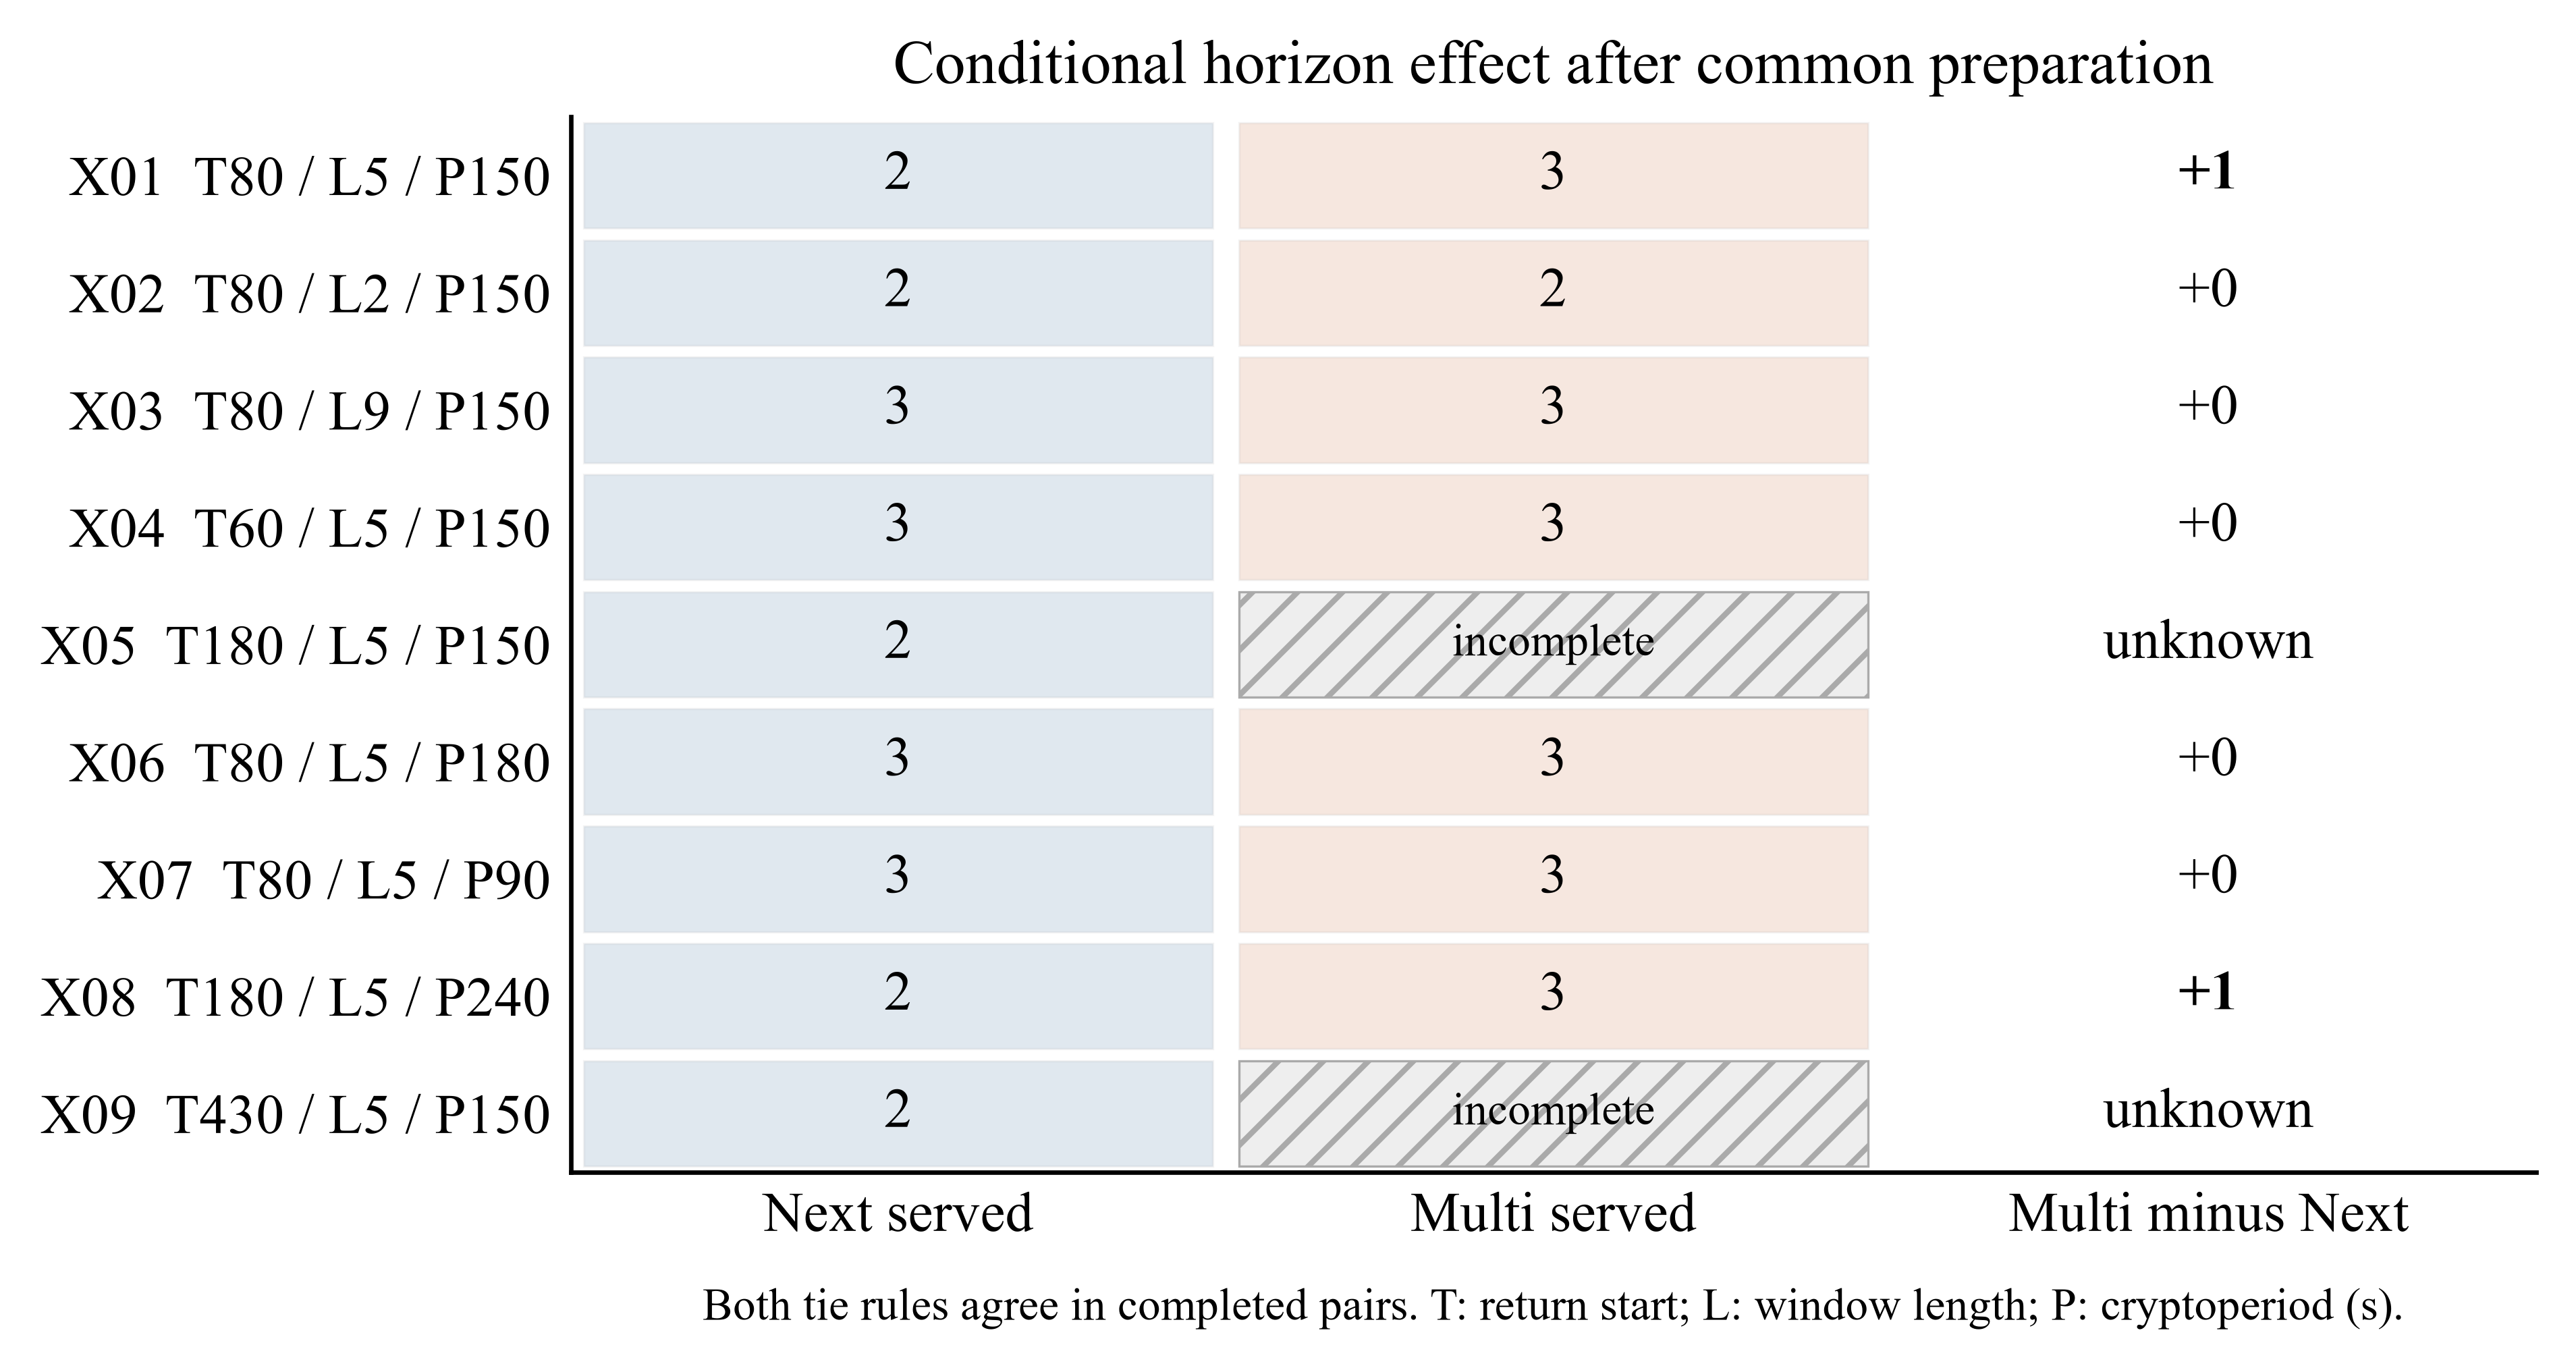
\includegraphics[width=\linewidth]{figures/horizon_conditions.png}
\caption*{Fig. 1. Synthetic conditions after common preparation. T is return-contact start, L its length, and P cryptoperiod, all in seconds. Both tie rules agree in completed pairs. Hatched cells are incomplete exact executions, not zero service.}
\end{figure}
A two-second return window is insufficient for the considered entry chains. A nine-second window allows later installation and both horizons serve three contacts. Returning at 60 seconds or extending the cryptoperiod to 180 seconds preserves useful old material and removes the difference. With P=90, expiry inside C1 forces even Next to renew, also removing the difference. At T=180 and P=240, earlier installation again enables a third contact only for Multi. At T=430 all material created by C1's end has exceeded its 400-second age limit before return, but the full policy comparison remains unknown because search is incomplete. The family establishes conditional examples, not a general interval threshold.

\subsection*{Quality and computational budget}
All 26 new budget attempts finish. Fig. 2 shows no offline horizon advantage in either workload at any tested allowance. For X, no DFS yields (2, 38, 0.32, 160, 2), whereas every positive node allowance yields (2, 38, 0.12, 160, 0): search avoids unused preparation without recovering C3. The long-window control gives (3, 410, 2.13, 3240, 6) for both horizons at every level.

\begin{figure}[htbp]\centering
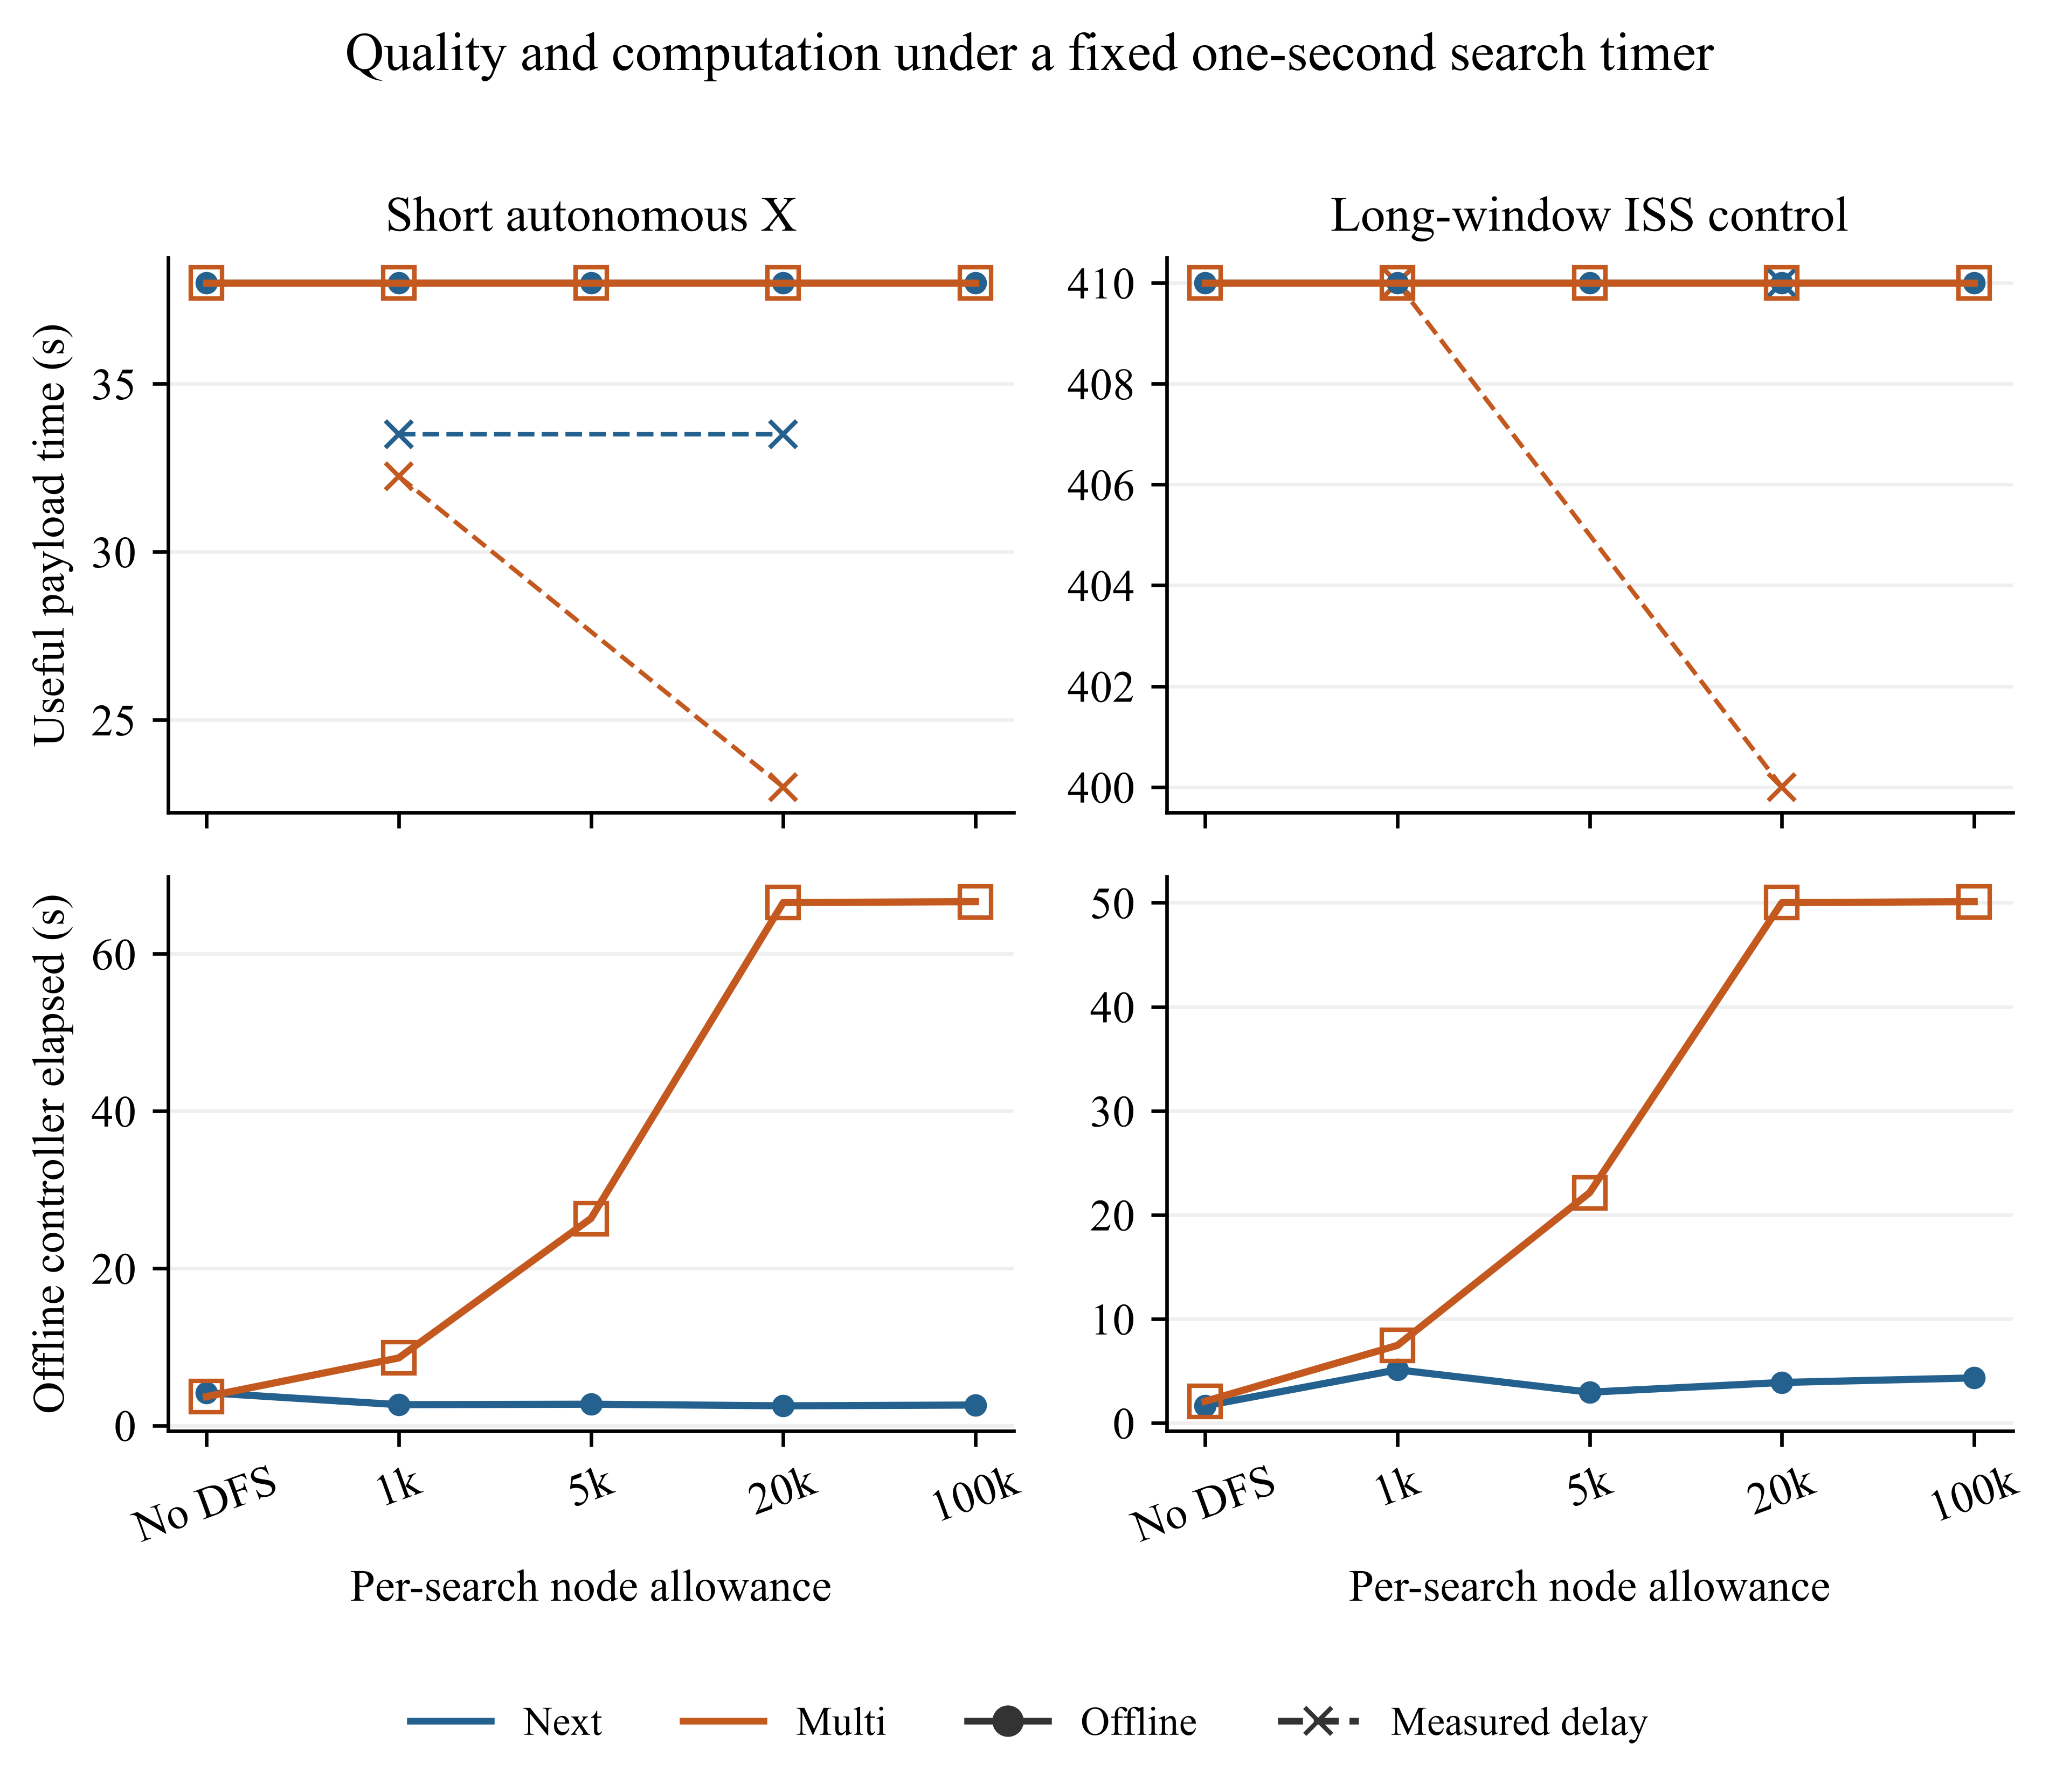
\includegraphics[width=\linewidth]{figures/quality_budget.png}
\caption*{Fig. 2. Full-run payload and host cost for CANONICAL. No DFS keeps seeds and retention. Crosses show selected measured-delay runs. Node values are allowances; time-limited decisions need not use them fully. Lines connect tested settings and imply no interpolation or statistical trend.}
\end{figure}
Larger allowances increase Multi's host cost without improving these offline scores. In X, its 20,000-node run contains 63 time-limited searches and totals about 66.5 seconds of controller time; the 100,000-node run also has 63 time-limited searches. The long control has 48 time-limited searches at each of these levels and about 50 seconds of controller time. Consequently, these observations do not test unconstrained use of the nominal node allowance. At 5,000 nodes, X's Multi controller takes about 26 seconds compared with roughly three seconds for Next, despite identical mission scores.

Charging decision latency produces three worse Multi outcomes and one tie across four paired settings. X useful time changes from Next/Multi 33.5/32.25 seconds at 1,000 nodes to 33.5/23 seconds at 20,000. In the long control the corresponding values are 410/410 and 410/400 seconds. Contact counts remain equal within each pair. No practical horizon gain is established by this budget series; a larger search allowance does not guarantee a better full receding-horizon execution.

\subsection*{Sensitivity to disclosure timing and tie order}
All 36 disclosure attempts finish, have a valid disclosed target, and eventually deliver an independent frame. There are no censored observations in this new grid. Fig. 3 compares matched horizons. CANONICAL gives earlier independent delivery for Multi in seven of nine timing pairs and 1,000 additional confidential bytes in five. CONTINUE\_WAIT gives equal independent-delivery times and confidential bytes in all nine pairs. Neither pattern establishes robustness to untested tie orders.

\begin{figure}[htbp]\centering
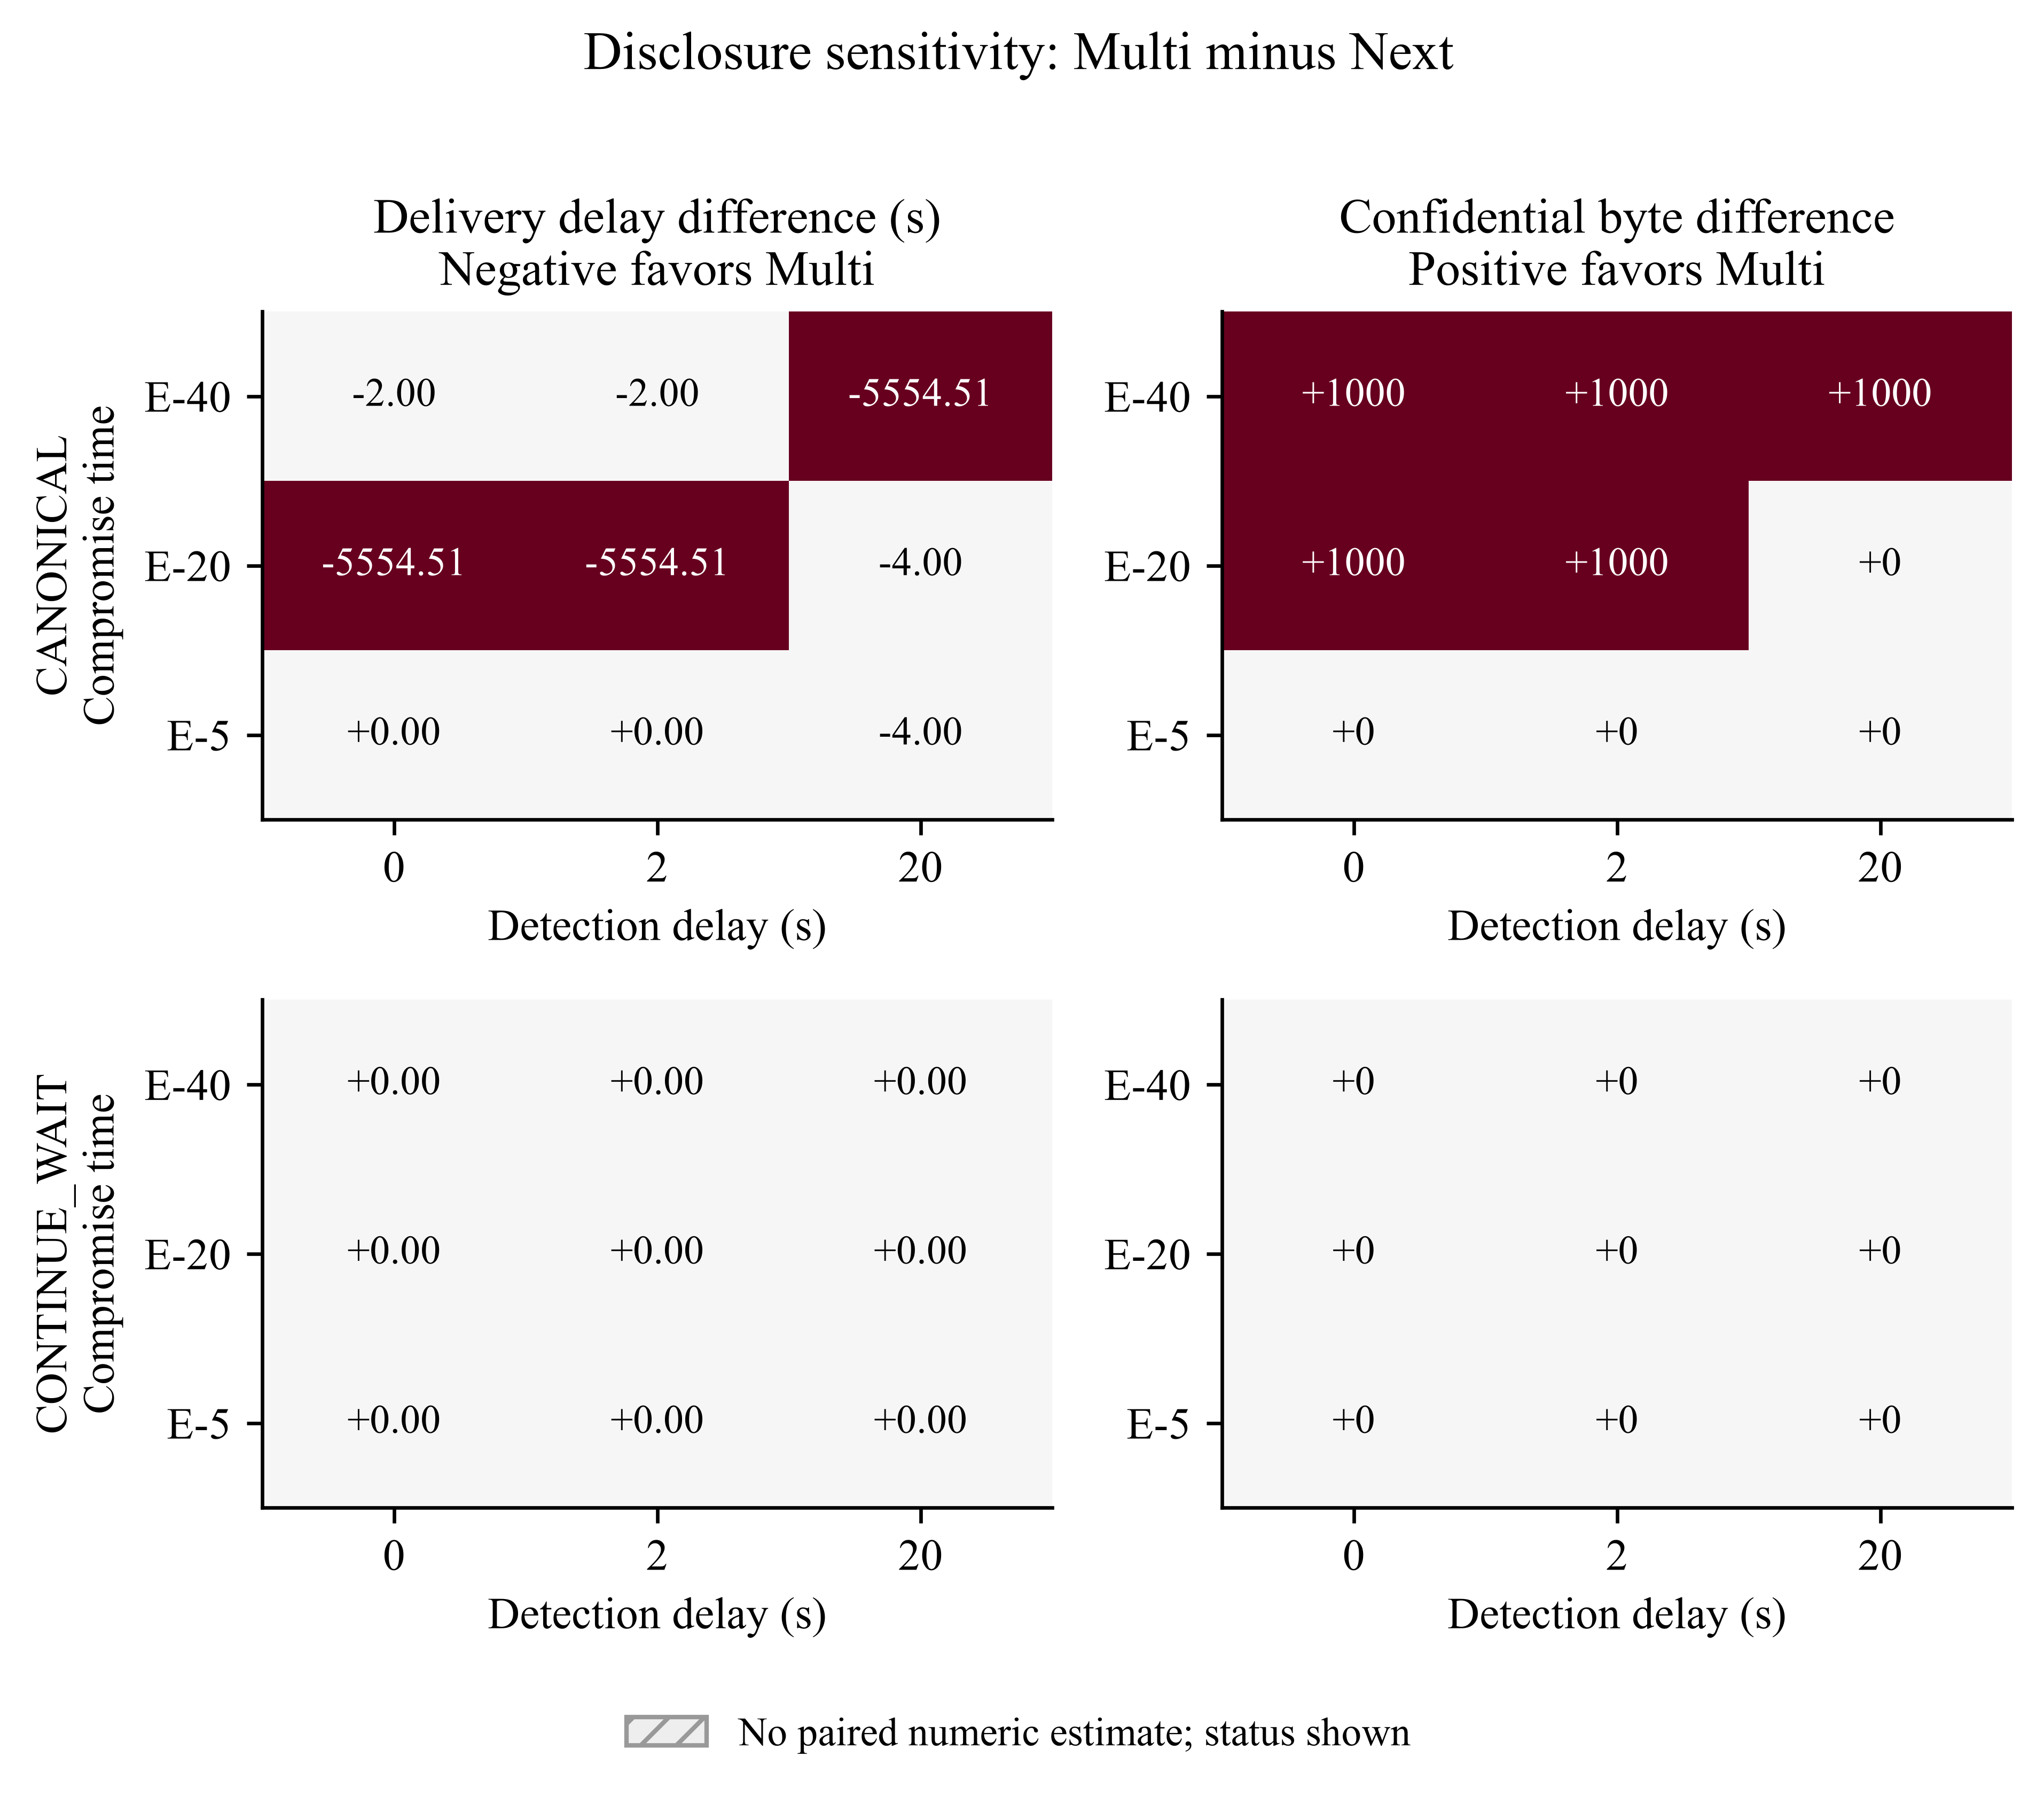
\includegraphics[width=\linewidth]{figures/disclosure_sensitivity.png}
\caption*{Fig. 3. Multi minus Next for first independent delivery delay and confidential delivered bytes, separated by tie rule. E is contact end; rows are common compromise times and columns detection delays. All 36 runs finished and recovered. Signed values are per-pair differences, not means over selected successes.}
\end{figure}
The largest delay difference is about 5,554.5 seconds: under CANONICAL, fitting one independent frame before contact loss avoids waiting for the next return. This occurs at E$-$40 with a 20-second detection delay, and E$-$20 with zero or two seconds of delay. The effect combines horizon-dependent state and tie-dependent action timing. All runs serve three contacts by the original service definition, which must not be confused with confidentiality.

Early activation is not equivalent to early delivery. At E$-$5 with immediate detection, CANONICAL Multi activates independent generation g2 after 1.4 seconds, but its 5,400-second cryptoperiod expires before return. Generation g3 supplies the first independent frame after 5,559.212 seconds, exactly when Next delivers. Multi uses eight new directional keys versus Next's six and delivers 400 rather than 410 useful seconds; both deliver 4,000 confidential bytes. The readiness-interval audit therefore rejects an inference of continuous readiness from the first activation milestone.

\section*{Discussion}
The experiments support the proposed timing mechanism in a restricted, explicit setting. Extra forecast information is useful when it exposes a later requirement early enough to change current lifecycle work, the resulting material survives until use, and the controller discovers and executes the necessary continuation. Holding only the action set constant is insufficient: initial preparation, complete plan tie order, and computational budget also change what the realized controller can achieve.

The preserved baseline explains why a mechanism witness did not translate into a main-matrix Multi advantage. Its practical core contains 54 attempts, of which 46 finish and eight time out. Among nine matched nominal Next/Multi cases, four pairs complete and tie on all five criteria; five remain incomplete. Main-profile windows leave enough time for later security work, and many same-context return gaps exceed the 5,400-second cryptoperiod. With initially empty keys, positive uplink/downlink service thresholds, and no admissible reuse across served returns, each served contact requires two fresh directional keys, giving (3). This conditional count does not establish optimality for useful time, CPU, bytes, or search cost.

\begin{equation}K_{\mathrm{new}}\geq 2S\tag{3}\end{equation}
The lower bound applies only when the stated initial-state and reuse assumptions hold. Pre-existing suitable material, longer valid reuse, or different directional demand can invalidate it. In the baseline, longer-cryptoperiod sensitivity permits reuse for both horizons rather than creating an exclusive Multi benefit. Geometric-window results also remain specific to modeled payload, station access, and costs. The four complete nominal pairs cannot resolve the five unfinished comparisons or all orbital environments.

The synthetic 4-versus-8-second entry arithmetic helps identify a testable mechanism but is not a new general scheduling theorem. It differs from the 22-versus-26-second totals in the baseline payload profile, and neither total alone proves that a plan meets event boundaries and key validity. Similarly, retaining a proved suffix is sound only under its guarded state and horizon conditions; it is not a blanket license to skip replanning after attacks or unforeseen changes.

The disclosure findings reinforce the separation between efficiency and security consequences. The objective rewards service and low overhead, not minimal exposure. A plan that renews earlier can waste key material before return, and additional useful time can include traffic later revealed. Reporting independent activation, delivery, and confidential bytes prevents a quick key replacement from being mistaken for faster end-to-end recovery. The selected late-disclosure grid tests one workload and active-pair threat model, not the probability of attack or resistance of a cryptographic protocol.

The study remains bounded by synthetic costs, discrete start opportunities, limited forecast horizons, nominal future operations, and host-specific timing. Exact results are finite-model root optima, whereas practical results are feasible outcomes under registered limits. The nine configurations and 36 disclosure runs were selected before outcomes but are not a statistical population sample. The unresolved exact cells, timer-constrained budget levels, and tie-dependent recovery benefits are substantive limits on the research conclusion, not missing values to be filled with optimistic estimates.

\section*{Conclusion}
Joint planning of directional keys and security associations across predicted contacts can preserve an otherwise missed contact. The new matched experiments establish this in two synthetic configurations under both tested tie rules and show why the effect disappears in five others. They also isolate an autonomous continuation that passes ordinary feasibility and evaluation checks but is not discovered by the bounded practical search. These findings support a conditional scheduling contribution rather than universal superiority of a longer horizon.

No practical horizon advantage appears in the tested offline budget series, and charged computation produces three losses and one tie. Disclosure benefits depend on tie order, and early independent activation can expire without accelerating delivery. The resulting research claim is therefore about the interaction of contact timing, material validity, plan selection, and computation. Unfinished comparisons remain unresolved; neither cryptographic security nor mission-wide optimality is proved.

\section*{Acknowledgments and declarations}
Funding, acknowledgments, competing interests, and corresponding-author designation: [AUTHOR TO CONFIRM]. No human or animal participant study was conducted; this work uses simulation and archived orbital/station inputs.

Data and code availability: the prior final-v2 reproduction package is publicly available at \url{https://github.com/MuhammedZhumali/ContactAwareSSGS/releases/tag/research.} The present revision supplies separate registered inputs, journals, diagnostics, audited tables, plotting and authoring scripts, and a manifest. It has not yet been deposited at a public persistent URL; the baseline release must not be cited as containing these new experiments. Supplementary material documents run origins, limits, recovery intervals, and unresolved comparisons.

\section*{References}
\noindent\hangindent=0.7cm [1] Consultative Committee for Space Data Systems. (2022). \textit{Space data link security protocol} (CCSDS 355.0-B-2). \url{https://ccsds.org/Pubs/355x0b2.pdf}\par
\noindent\hangindent=0.7cm [2] Consultative Committee for Space Data Systems. (2020). \textit{Space data link security protocol---Extended procedures} (CCSDS 355.1-B-1). \url{https://ccsds.org/Pubs/355x1b1.pdf}\par
\noindent\hangindent=0.7cm [3] Consultative Committee for Space Data Systems. (2023). \textit{Symmetric key management} (CCSDS 354.0-M-1). \url{https://ccsds.org/Pubs/354x0m1.pdf}\par
\noindent\hangindent=0.7cm [4] Consultative Committee for Space Data Systems. (2019). \textit{Schedule-aware bundle routing} (CCSDS 734.3-B-1). \url{https://ccsds.org/Pubs/734x3b1.pdf}\par
\noindent\hangindent=0.7cm [5] Fraire, J. A., De Jonckère, O., \& Burleigh, S. C. (2021). Routing in the Space Internet: A contact graph routing tutorial. \textit{Journal of Network and Computer Applications, 174}, Article 102884. \url{https://doi.org/10.1016/j.jnca.2020.102884}\par
\noindent\hangindent=0.7cm [6] Burleigh, S., Horres, D., Viswanathan, K., Benson, M., \& Templin, F. (2018). \textit{Architecture for delay-tolerant key administration} (Internet-Draft draft-burleigh-dtnwg-dtka-02) [Expired draft]. Internet Engineering Task Force. \url{https://datatracker.ietf.org/doc/html/draft-burleigh-dtnwg-dtka-02}\par
\noindent\hangindent=0.7cm [7] Fuchs, F., Walter, F., \& Tschorsch, F. (2025). BERMUDA: A BPSec-compatible key management scheme for DTNs. In L. Nemec Zlatolas, K. Rannenberg, T. Welzer, \& J. Garcia-Alfaro (Eds.), \textit{ICT systems security and privacy protection} (IFIP Advances in Information and Communication Technology, Vol. 746, pp. 219--233). Springer. \url{https://doi.org/10.1007/978-3-031-92886-4_15}\par
\noindent\hangindent=0.7cm [8] Zhao, H. (2020). A context-based secure handover mechanism for space-ground-integrated network. \textit{Research Briefs on Information and Communication Technology Evolution, 6}, 52--61. \url{https://doi.org/10.56801/rebicte.v6i.94}\par
\noindent\hangindent=0.7cm [9] Kwon, D. K., Son, S., Park, K., Das, A. K., \& Park, Y. (2025). An efficient handover authentication scheme for 6G-enabled space-terrestrial integrated networks with mobile edge computing. \textit{IEEE Transactions on Information Forensics and Security, 20}, 12157--12172. \url{https://doi.org/10.1109/TIFS.2025.3628470}\par
\noindent\hangindent=0.7cm [10] Bernal, D., Ledesma, O., Lamo, P., \& Bermejo, J. (2026). IOTA-based authentication for IoT devices in satellite networks. \textit{Computers, Materials \& Continua, 86}(1), 1--39. \url{https://doi.org/10.32604/cmc.2025.069746}\par
\noindent\hangindent=0.7cm [11] Burleigh, S., Fall, K., \& Birrane, E., III. (2022). \textit{Bundle protocol version 7} (RFC 9171). RFC Editor. \url{https://doi.org/10.17487/RFC9171}\par
\noindent\hangindent=0.7cm [12] Birrane, E., III, \& McKeever, K. (2022). \textit{Bundle protocol security (BPSec)} (RFC 9172). RFC Editor. \url{https://doi.org/10.17487/RFC9172}\par
\noindent\hangindent=0.7cm [13] Detke, R., Madoery, P. G., Cherini, R., Fraire, J. A., \& Finochietto, J. M. (2026). \textit{Security-aware route selection in DTNs: Towards optimal key provisioning} [Conference paper]. Space-Terrestrial Internetworking Workshop, IEEE WiSEE. \url{https://stintworkshops.org/papers/stint2026-19-detke.pdf}\par
\noindent\hangindent=0.7cm [14] Mattingley, J., Wang, Y., \& Boyd, S. (2010). Code generation for receding horizon control. In \textit{2010 IEEE International Symposium on Computer-Aided Control System Design} (pp. 985--992). IEEE. \url{https://doi.org/10.1109/CACSD.2010.5612665}\par
\noindent\hangindent=0.7cm [15] Dowling, B., Hale, B., Tian, X., \& Wimalasiri, B. (2025). Cryptography is rocket science: Analysis of BPSec. \textit{IACR Communications in Cryptology, 1}(4). \url{https://doi.org/10.62056/a39qudhdj}\par
\noindent\hangindent=0.7cm [16] Madoery, P. G., Cherini, R., Cammarano, A., Grosso, J., \& Finochietto, J. M. (2024). Bundle protocol security models and policies for safeguarding space information networks. \textit{IEEE Journal of Radio Frequency Identification, 8}, 547--558. \url{https://doi.org/10.1109/JRFID.2024.3406890}\par
\noindent\hangindent=0.7cm [17] Birrane, E., III, White, A., \& Heiner, S. (2022). \textit{Default security contexts for Bundle Protocol Security (BPSec)} (RFC 9173). RFC Editor. \url{https://doi.org/10.17487/RFC9173}\par
\noindent\hangindent=0.7cm [18] Kelso, T. S. (2026, June 23). \textit{A new way to obtain GP data (aka TLEs)}. CelesTrak. \url{https://celestrak.org/NORAD/documentation/gp-data-formats.php}\par
\noindent\hangindent=0.7cm [19] Libre Space Foundation. (n.d.). \textit{API}. SatNOGS Network documentation. Retrieved October 28, 2026, from \url{https://docs.satnogs.org/projects/satnogs-network/en/stable/api.html}\par
\noindent\hangindent=0.7cm [20] Orekit. (n.d.). \textit{Orekit}. Retrieved October 28, 2026, from \url{https://www.orekit.org/}\par
\end{document}
